\chapter*{Appendix: i-Vector/PLDA speaker recognition}
\label{appendix:ivector_plda_spkr_id}

This appendix is presented for the curious reader who is interested in becoming more familiar with the i-Vector/PLDA speaker recognition platform. 
This is in no means a comprehensive introduction for this type of system, rather its function is to provide context for proposed systems in Chapter~\ref{chapter:backend}. 
Speaker recognition in i-Vector/PLDA system is implemented in a way to fall in the speaker verification framework. 
Much like a GMM-UBM system, each decision provides a likelihood ratio verifying whether a train speaker matches audio from a test speaker. 
An i-Vector/PLDA system typically trains a speaker model (i.e., i-Vector) using multiple training files. 
Unlike GMM-UBM, test speakers are also represented by speaker models. 
Therefore, train and test speakers are treated similarly in an i-Vector/PLDA system. 
Figure~\ref{fig:ivector_plda} summarizes a typical i-Vector/PLDA system~\cite{dehak2011front}. 

\renewcommand{\thefigure}{A.\arabic{figure}}
\setcounter{figure}{0}
\begin{figure}[h!]
	\centering
	\vspace{0mm} 
	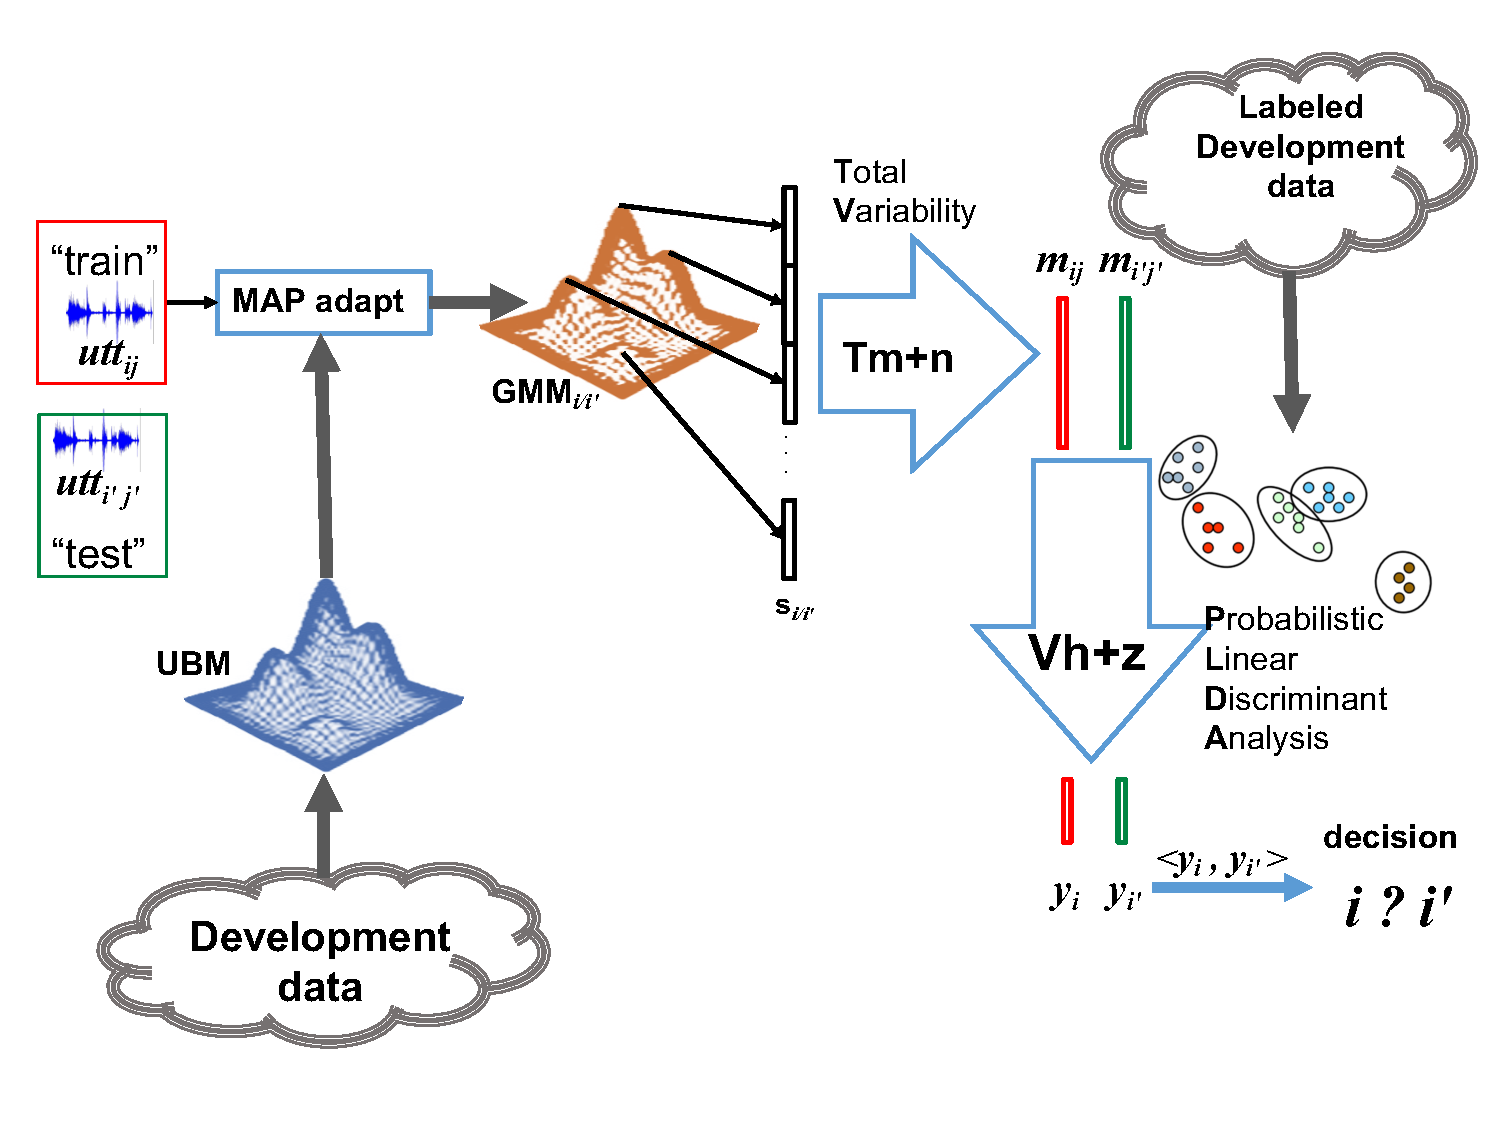
\includegraphics[height = 4in, width=0.9\textwidth]{figures/ivector_plda}
	\vspace{-3mm}
	\caption{Overview of i-Vector/PLDA system.}
	\label{fig:ivector_plda}
	\vspace{-3mm}
\end{figure}

The first step is extract to i-Vectors from a collection of audio files (or a single audio file), provided for each speaker. 
i-Vectors are obtained by compressing Gaussian mean super-vectors. 
Super-vectors are a concatenation of GMM means. 
Since GMMs are typically composed of 512 (or more) Gaussian mixtures, the concatenated GMM means result in incredibly large super-vectors (36-dimensional MFCC means $\times$ 512 Gaussian mixtures). 
Therefore, i-Vectors can be viewed as a dimension reduction technique to reduce the dimension of super-vectors. 
This is done through a factor analysis process that represents super-vectors as factor loadings of a Total Variability (TV) matrix. 
The factor loading weights are called i-Vectors (denoted ${\bf m}$ in Fig.~\ref{fig:ivector_plda}). 
TV matrix can be trained using unlabeled development data (typically the same data used to train the UBM). 

An i-Vector is provided for the train and test components in each trial. 
The next step is to compare these two i-Vectors to determine whether they represent the same speaker. 
Many methods have been proposed to compare i-Vectors, the most popular of which is probabilistic linear discriminant analysis (PLDA). 
PLDA has been thoroughly explained in Chapter~\ref{chapter:backend}, but it can also be viewed as a factor analysis method to remove certain (unwanted) variabilities from the i-Vectors. 
The likelihood ratio provided by PLDA is typically used to determine the certainty to which the system believes the two i-Vectors from a trial belong to the same speaker. 
